
%==========================================================
\section{Introduction}

\section{Nomenclatures}

\begin{table}[!htb]

  \centering
  \begin{tabular}{||l|c||}
    \hline
    $P$   & Population \\
    \hline
    $\text{GDP}$ & Gross Domestic Product \\
    \hline
    $\text{PCGDP}$ & Per Capita Gross Domestic Product \\
    \hline
    $\text{GAP}$ & Cross Agricultural Product \\
    \hline
    $\text{AWC}$ & Agricultural Water Consumption per year \\
    \hline
    $\text{IWC}$ & Industrial Water Consumption per year \\
    \hline
    $\text{DWC}$ & Domestic Water Consumption per year \\
    \hline
    $\text{TWR}$ & Total Water Resource \\
    \hline
    $\text{SWR}$ & total Surface Water Resource \\
    \hline
    $\text{UWR}$ & total Underground Water Resource \\
    \hline
    $\text{PCGDP}$ & Per Capita Gross Domestic Product \\
    \hline
    $\text{IA}$ & Irrigation Area \\
    \hline
    $\text{ISP}$ & Iron and Steel Production \\
    \hline
    $\text{ElP}$ & Electricity Production. \\
    \hline
    $\text{EnC}$ & Engel's Coefficient \\
    \hline
    $A$          & Annual water supplies per person \\
    \hline
  \end{tabular}
  \caption{Nomenclatures System}
  \label{tab: Nomenclatures sys}
\end{table}

\section{Model of water supply ability}
  When it come to the water supply ability of a region, a country or even the world. We often use the measurement called annual water supplies per person($A$) for description\cite{AbilityMeasure}. We can set three levels to classify the ability of several regions:
  \begin{table}[!htb]
    \centering
    \begin{tabular}{|c||c|c|}
    \hline
    level 1   & $A>1700$ & Sufficient \\
    \hline
    level 2   & $1700>A>1000$ & stressful \\
    \hline
    level 3   & $1000>A$ & scarce \\
    \hline
    \end{tabular}
    \caption{water supply ability}
  \end{table}

To cover the internal dynamics of the water flow and the water storage change, we introduce following model.

  \subsection{Model Introduction}
    Water circulation is a rather complicated process, which make it almost impossible for us to design a purely fundamental model to include all the variables and their relations. Nevertheless, if we just collect all the data and using fitting method as our predicting model, it will be too trivial and old-fashioned. To solve this paradox, we introduce a phenomenological model which is quite normal in particle physics and other related field. Our model includes two main parts:
    \begin{itemize}
      \item prominent external parameters: a several statistical parameters about a region like population, GDP and so on.
      \item internal dynamic variables: find out the relation between prominent external parameters and internal variables including Agriculture Water Consumption, Industrial Water Consumption and Domestic Water consumption.
    \end{itemize}
    The prominent external parameters comes from the statistic numbers and it's fitness, while the internal dynamics variables is mainly based on prominent parameters, which makes them indirectly depend on time in our model.

  \subsection{Model Structure}

    \begin{figure}[!h]
    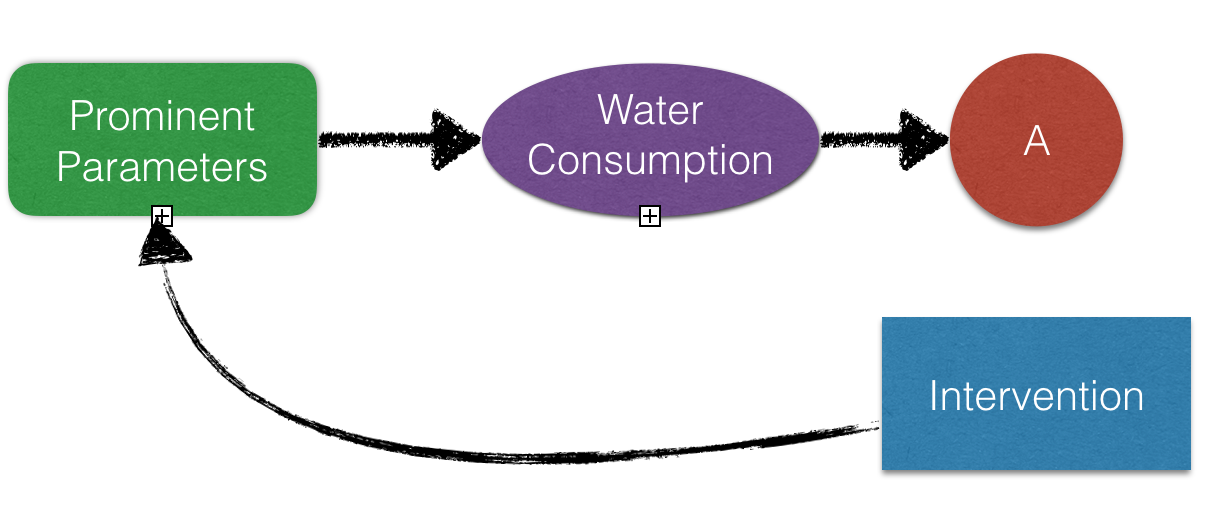
\includegraphics[width = 0.9\textwidth]{picture/struct.png}
    \caption{structure}
    \label{fig: structure}
    \end{figure}
    Our model's structure is pretty clear.
    We using some prominent external parameters as the input of our dynamic system. To determine the water supply ability of a region, the most important part is the water flow which means the total amount of industrial, agricultural and residential consumption. The season we can use the consumption to measure the supply it that they must be the same during a long period just like the electricity use equal to the electricity produce.

    $$
    \langle \text{Consumption}\rangle = \langle \text{Supply} \rangle
    $$

    The $W$ and $\bar{W}$ is a crucial conception in our dynamic part, $W$ stand for the total clean water resource over a period, while the $\bar{W}$ is the total wasted water resource which can be transfered into $W$ after several processing steps.

  \subsection{Model Prominent Parameters}

    The prominent parameters are some thing the dynamics part heavily rely on, to find the prominent parameters, we need to investigate the relation between some alternative parameters and consumptions according to the past data. In other words, prominent parameters are not given before a specific research object is given, we just give some alternative parameters and using the past data to determine which is better related and which is less related to our dynamic part variables.

    Generally, there are several important alternative parameters like: Population, GDP Per Capita are of course important statistic numbers. Moreover, Agricultural Irrigation Area play an important role in agricultural consumption, Iron and Steel Production is also important in industrial consumption, and Engel's coefficient is an important statistical number about residential living which make it important in residential consumption.

  \subsection{Model Dynamics}

    \begin{wrapfigure}{l}{8cm}
    %\begin{center}
    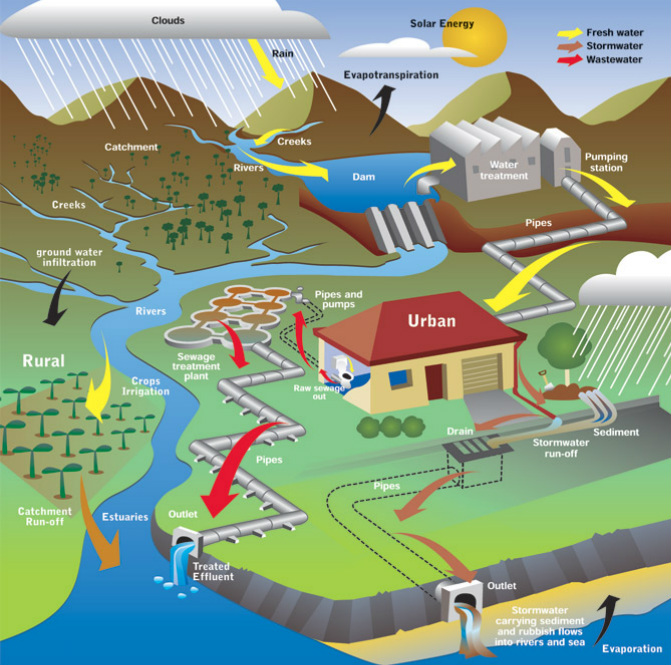
\includegraphics[width = 8cm]{picture/UrbanWaterCycle.jpg}
    \caption{water cycle\cite{WaterCycle}}
    \label{water cycle}
    %\end{center}
    \end{wrapfigure}
    The dynamics part of our model is inspired by the water cycle(Figure ~\ref{water cycle}). Basically, our water is mainly refreshed though the precipitation. So it will be elegant if we using such water cycle process to build a mighty system about how the water flow and run with real data to determine the theoretical water consumption. However, after several data browse, we find that using precipitation as part of the water storage's changing rate is ridiculous--The total water resource is steadily a certain ratio of precipitation. Therefore using prominent parameters as arguments of internal variables and find the relation according to the past data will be a proper choice.

  \subsection{How to apply our model}

    With good structure of our model and program, the application of our model can be done in a pretty clear way.

    \begin{enumerate}[step 1]
      \item Using the past data of alternative prominent parameters, find proper relation between those parameters and time, therefore determine the time dependent equation of prominent parameters.
      \item Using the data of alternative prominent parameters and consumption variables in the past to find the strength of correlation, Spearman or Pearson or other coefficients.
      \item According to the coefficients, structure the parameter dependent equations of consumption variables.
      \item With the equations construed above and the time dependent equation of prominent parameters, get the tendency of consumption variable therefore getting the prediction of water consumption and the water supply per person ($A$).
    \end{enumerate}



\section{China's water scarcity}
  According to the UN water scarcity map, China is a country with water stress,
  \begin{wrapfigure}{l}{7cm}
  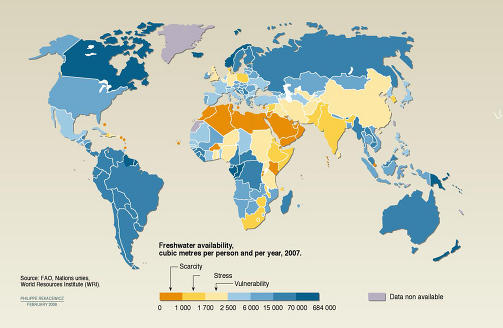
\includegraphics[width = 6cm]{picture/WaterScarcityMap.jpg}
  \caption{water scarcity map\cite{WaterScarcityMap}}
  \end{wrapfigure}
  which make it a region where water is moderately overloaded. In our consideration, level 2, will provide more abundant behavior in a dynamical model(will it become water scarce or water sufficient in the future?). Thus we pick up China as our research object. To make our model more predictable and more reality connected.
  \clearpage
  \subsection{Social drivers}
  demo demo demo demo demo demo demo demo demo demo demo demo demo demo demo demo demo demo demo demo demo demo demo demo demo demo demo demo demo demo demo demo demo demo demo demo demo demo demo demo demo demo demo demo demo demo demo demo demo demo demo demo demo demo demo demo demo demo demo demo demo demo demo demo demo demo demo demo demo demo demo demo demo demo demo demo demo demo demo demo demo demo demo demo demo demo demo demo demo demo demo demo demo demo demo demo demo demo demo demo demo demo demo demo demo demo demo demo
  \subsection{Environmental drivers}
  demo demo demo demo demo demo demo demo demo demo demo demo demo demo demo demo demo demo demo demo demo demo demo demo demo demo demo demo demo demo demo demo demo demo demo demo demo demo demo demo demo demo demo demo demo demo demo demo demo demo demo demo demo demo demo demo demo demo demo demo demo demo demo demo demo demo demo demo demo demo demo demo demo demo demo demo demo demo demo demo demo demo demo demo demo demo demo demo demo demo demo demo demo demo demo demo demo demo demo demo demo demo demo demo demo demo demo demo demo demo demo demo demo demo demo demo demo

\section{China's water scarcity: Further Investigation and Prediction}

  For further investigation, we study with the data from National Bureau of Statistics of the People's Republic China\cite{ChinaDataBase}.According to our models, we should predetermine the alternative prominent parameters and grab all the data and try to analyses them and they relation.
  \subsection{Prominent variables' tendency}
  Using proper assumption and the past data in databases. We can using fitness method to determine the time dependency of our alternative parameters.
  In our consideration, following factors especially eye-catching.
  \begin{table}[!h]
  \centering
  \begin{tabular}{|c|c|}
  \hline
  $P$ & Population \\
  \hline
  $\text{PCGDP}$ & Per Capita Gross Domestic Product \\
  \hline
  $\text{IA}$ & Irrigation Area \\
  \hline
  $\text{ISP}$ & Iron and Steel Production \\
  \hline
  $\text{ElP}$ & Electricity Production. \\
  \hline
  $\text{EnC}$ & Engel's Coefficient \\
  \hline
  \end{tabular}
  \end{table}
  For further convenience, we will investigate their relation towards time at first.
    \paragraph{Population}
      The population growth model is various, for best concern, we use Logistic Model as the Population evolution model thus we can use the solution--Standard logistic sigmoid function as our target function by adding three basic coefficients.
      $$
      P(t) = \frac{K^P}{1+\exp[-\lambda^P(t-t_0^P)]}
      $$

    \paragraph{Per Capita Gross Domestic Product}
      As the largest developing country over the world, China has pretty high PCGDP growth rate. It seems like an exponential growth However, according to our data browse, some developed countries have already reach some obstacles. Thus we think it will be suitable if we apply Logistic model in the fitness model of $\text{PCGDP}$.
      $$
      \text{PCGDP}(t) = \frac{K^\text{PCGDP}}{1+\exp[-\lambda^\text{PCGDP}(t-t_0^\text{PCGDP})]}
      $$

    \paragraph{Irrigation Area}
      According to our observation, there is a strong evidence about linear growth of Irrigation Area. Consider the complicity and the fact we are just required to predict about 15 years, a polynomial fitting with power 2 is sufficient.
    $$
    \text{IA}(t) = A_0^\text{IA}+A_1^\text{IA} t + A_2^\text{IA} t^2
    $$

    \paragraph{Iron and Steel Production}
      The data of ISP perform in a similar way of IA, therefore we can use the same method to predict the ISP evolution.
    $$
    \text{ISP}(t) = A_0^\text{ISP}+A_1^\text{ISP} t + A_2^\text{ISP} t^2
    $$

    \paragraph{Electricity Production}
      The behavior of ELP is every bit as same as two parameters above, thus we just apply the same evolution equation form.
    $$
    \text{ELP}(t) = A_0^\text{ELP}+A_1^\text{ELP} t + A_2^\text{ELP} t^2
    $$

    \paragraph{Engel's Coefficient}
      Engel's Coefficient perform in a much different way. When it comes to the Engel, it make sense that with the development of society. It will keep decreasing as it used to be with a limit target: zero. Therefore we introduce a inverse proportion function to describe it's tendency.
    $$
    \begin{cases}
    \text{Enc}_\text{urban}(t) = C^\text{urban}/(t-t_0^\text{urban}) \\
    \text{Enc}_\text{rural}(t) = C^\text{rural}/(t-t_0^\text{rural})
    \end{cases}
    $$


    \begin{figure}[!h]
    \begin{center}
    \subfigure[$p(t)$]{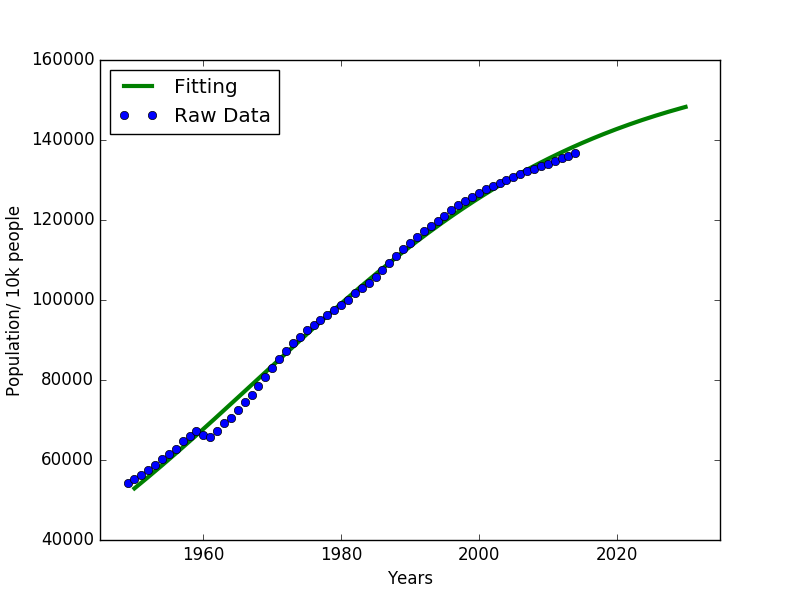
\includegraphics[width = 0.45\textwidth]{picture/Population.png}}
    \subfigure[$\text{PCGDP}(t)$]{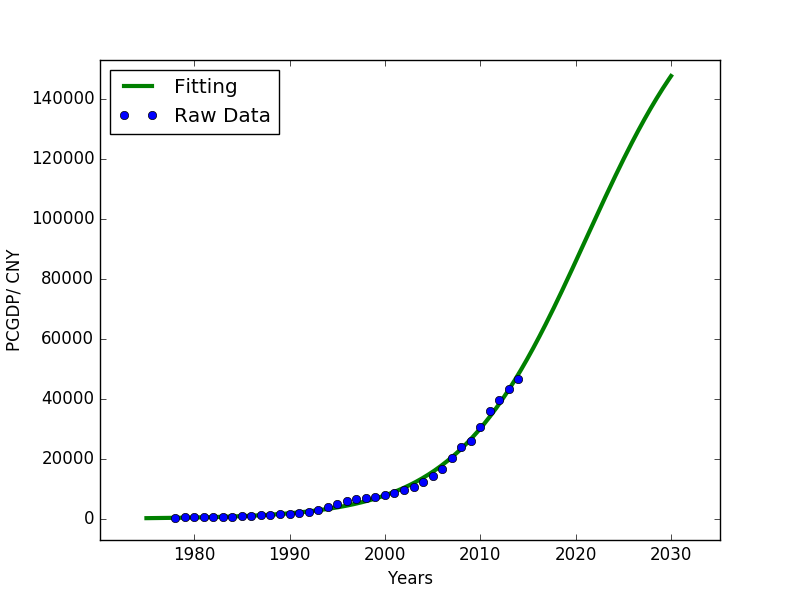
\includegraphics[width = 0.45\textwidth]{picture/PCGDP.png}}\\
    \subfigure[$\text{IA}(t)$]{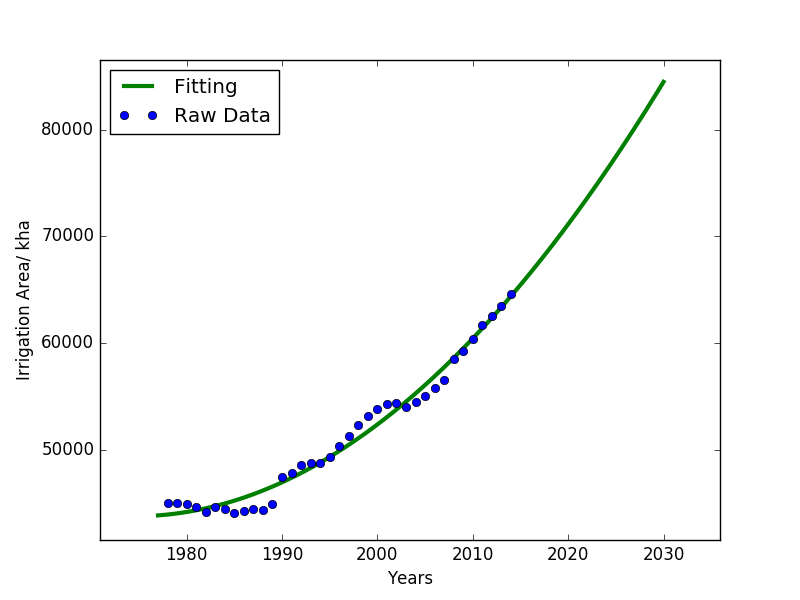
\includegraphics[width = 0.45\textwidth]{picture/IrrigationArea.png}}
    \subfigure[$\text{ISP}(t)$]{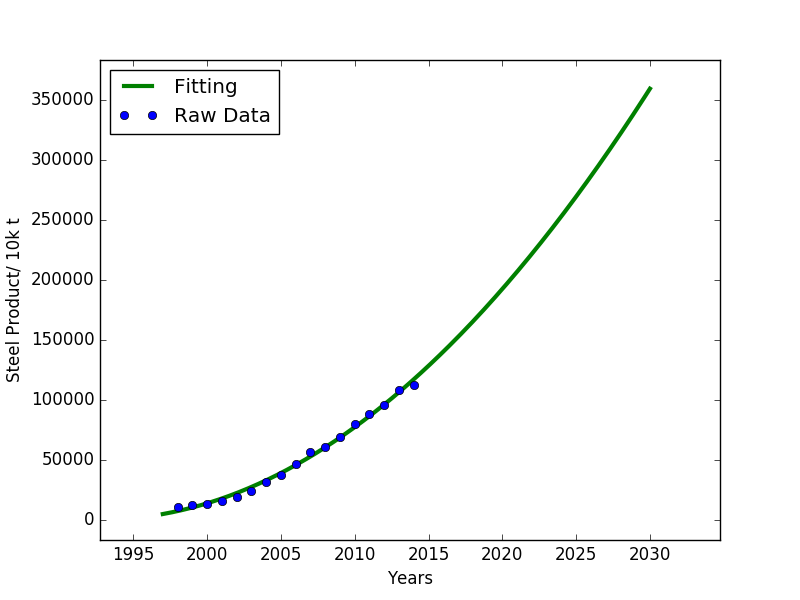
\includegraphics[width = 0.45\textwidth]{picture/SteelProduct.png}}\\
    \subfigure[$\text{ELP}(t)$]{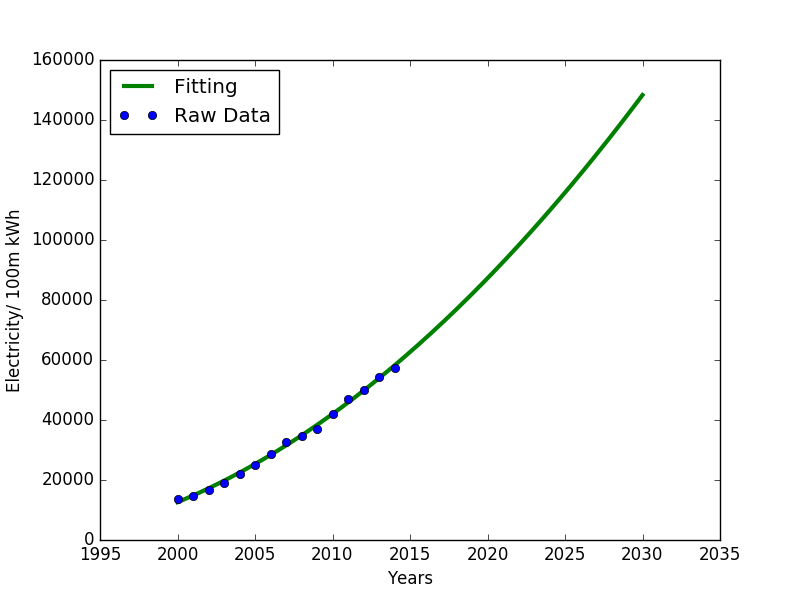
\includegraphics[width = 0.45\textwidth]{picture/Electricity.png}}
    \subfigure[$\text{Enc}(t)$]{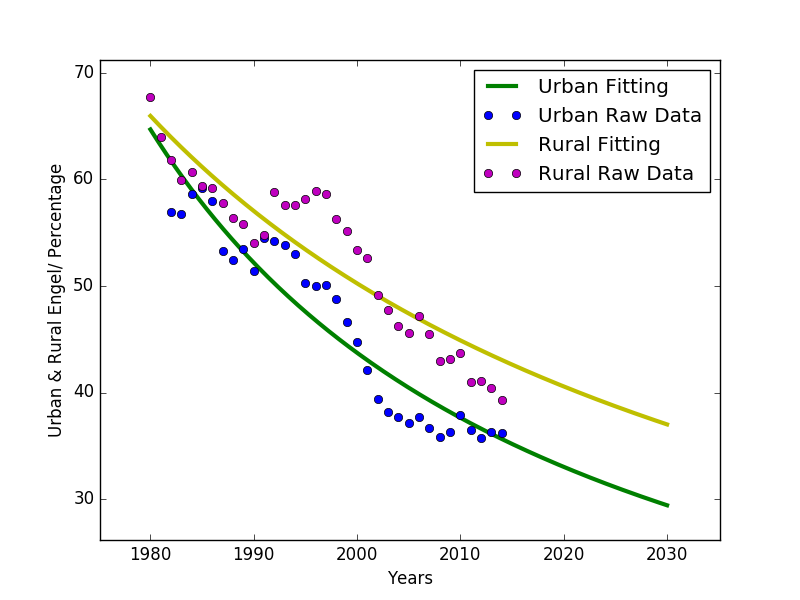
\includegraphics[width = 0.45\textwidth]{picture/Engel.png}}
    \end{center}
    \caption{Parameters fit: blue dots means the existed data which we refer from the national database, green lines stand for the optimized curve and the prediction value in the future }
    \label{fig: parameters fit}
    \end{figure}

    With the fitness method, we can get all the evolution of alternative prominent parameters in Figure ~\ref{fig: parameters fit}, and the parameters in evolution equations in Table~\ref{tab: evolution par}:
    \begin{table}[!h]
      \centering
      \begin{tabular}{|l|l|}
      \hline
      $\left[t_0^P, \lambda^P,K^P\right]$ & [1968.14, 3.94\%, 161162.404] \\
      \hline
      $\left[t_0^\text{PCGDP}, \lambda^\text{PCGDP},K^\text{PCGDP}\right]$ & [2021.12, 14.9\%, 187060.984] \\
      \hline
      $\left[A_0^\text{IA},A_1^\text{IA},A_2^\text{IA}\right]$ & [5.155e+07, -5.217e+04, 13.21] \\
      \hline
      $\left[A_0^\text{ISP},A_1^\text{ISP},A_2^\text{ISP}\right]$ & [1.027e+09, -1.031e+06, 258.6] \\
      \hline
      $\left[A_0^\text{ELP},A_1^\text{ELP},A_2^\text{ELP}\right]$ & [3.125e+08, -3.146e+05, 79.19] \\
      \hline
      $\left[C^\text{urban},t_0^\text{urban},C^\text{rural},t_0^\text{rural}\right]$ & [1938.24, 2700.15, 1916.02, 4218.31] \\
      \hline
      \end{tabular}
      \caption{evolution parameters}
      \label{tab: evolution par}
    \end{table}


  \subsection{Relation between prominent parameters and variables}
    To investigate the relation between prominent parameters and variables, we firstly introduce the conception of  correlation. In statistics, dependence is any statistical relationship between two random variables or two sets of data, and correlation refers to any of a broad class of statistical relationships involving dependence.


    \paragraph{Pearson product-moment correlation coefficient}\cite{Pearson} is a measure of the linear correlation between two variables $X, Y$. If there is two datasets $\{x_1,x_2,\dots, x_n\}$ and $\{y_1,y_2,\dots, y_n\}$, then the formula for r is\cite{pearsonr}:
    $$
    r = \frac{\sum{(x_i-\bar{x})(y_i-\bar{y})}}{\sqrt{\sum{(x_i-\bar{x})^2}}\sqrt{\sum{(y_i-\bar{y})^2}}}
    $$

    \paragraph{Spearman's rank correlation coefficient} is a nonparametric measure of statistical dependence between two variables. It assesses how well the relationship between two variables can be described using a monotonic function. If there are no repeated data values, a perfect Spearman correlation of $+1$ or $-1$ occurs when each of the variables is a perfect monotone function of the other\cite{Spearman}\cite{spearmanr}. The Spearman correlation coefficient is defined as the Pearson correlation coefficient between the ranked variables\cite{ranked variable}. For a sample of size n, the n raw scores $X_i,Y_i$ are converted ranks $x_i, y_i$, and $\rho$ is computed from:
    $$
    \rho = 1 - \frac{6\sum{(x_i-y_i)^2}}{n(n^2-1)}
    $$

    \paragraph{Kendall rank correlation coefficient} is a statistic used to measure the association between two measured quantities. Let $(x_1, y_1),(x_2, y_2),\dots,(x_n, y_n)$ be a set of observations of the joint random variables $X$ and $Y$ respectively, such that all the values of $(x_i)$ and $(y_i)$ are unique. Any pair of observations $(x_i,y_i)$ and $(x_j, y_j)$, where $i\neq j$, are said to be concordant if the ranks for both elements agree: that is, if both $x_i > x_j$ and $y_i > y_j$ or if both $x_i < x_j$ and $y_i < y_j$. They are said to be discordant, if $x_i > x_j$ and $y_i < y_j$ or if $x_i < x_j$ and $y_i > y_j$. If $x_i = x_j$ or $y_i = y_j$, the pair is neither concordant nor discordant. Thus the $\tau$ coefficient is defined as\cite{Kendall}\cite{kendalltau}:
    $$
    \tau = \frac{(\text{number of concordant pairs}) - (\text{number of discordant pairs})}{\frac{1}{2} n (n-1)}
    $$

    Using coefficients above, we get a map about the relation between prominent parameters and consumption variables.

    \begin{table}[!htb]

      \centering
      \begin{tabular}{l||c|c|c|c}
      \hline
      Data                & Pearson $(r_p,p)$                        & Spearman $(r_s,p)$       & Kendall $(\tau, p)$ & Average \\
      \hline

      $\text{IWC}\sim P$ & (0.669,0.0245)                   &(0.627,0.0388)   &(0.455,0.0516)     &   0.584\\
      \hline
      $\text{IWC}\sim \text{PCGDP}$ &(0.614,0.0444)         &(0.627,0.0388)   &(0.455,0.0516)     &   0.565\\
      \hline
      $\text{IWC}\sim \text{ELP}$ &(0.648,0.0311)           &(0.627,0.0388)   &(0.455,0.0516)     &   0.577\\
      \hline
      $\text{IWC}\sim \text{ISP}$ &(0.653,0.0294)           &(0.627,0.0388)   &(0.455,0.0516)     &   0.577\\
      \hline\hline
      $\text{AWC}\sim P$ &(0.924,4.95e-5)                   &(0.927,3.97e-5)  &(0.782,0.000815)     &   0.878\\
      \hline
      $\text{AWC}\sim \text{PCGDP}$ &(0.936,2.28e-5)        &(0.927,3.97e-5)  &(0.782,0.000815)     &   0.882\\
      \hline
      $\text{AWC}\sim \text{IA}$ &(0.927,4.10e-5)           &(0.927,3.97e-5)  &(0.782,0.000815)     &  0.879 \\
      \hline\hline
      $\text{DWC}\sim P$ &(0.844,0.00108)                   &(0.836,0.00133)  &(0.745,0.00141)     &   0.808\\
      \hline
      $\text{DWC}\sim \text{PCGDP}$ &(0.806,0.00276)        &(0.836,0.00133)  &(0.745,0.00141)     &   0.796\\
      \hline
      $\text{DWC}\sim \text{Enc}_\text{urban}$ &(-0.785,0.00417) &(-0.809,0.00256) &(-0.600,0.0102)     &  -0.731 \\
      \hline
      $\text{DWC}\sim \text{Enc}_\text{rural}$ &(-0.419,0.199)   &(-0.315,0.345)   &(-0.204,0.383)     &   -0.313\\
      \hline

      \end{tabular}
      \caption{Coefficients: Coefficients of correlation in different standard}
      \label{tab: coefficients}
    \end{table}



  \subsection{Fitness method in consumption variables}
  To investigate the evolution of consumption variables, We first investigate the correlation between one specific consumption with one specific prominent parameters.

  \begin{table}[!h]

  \centering
  \begin{tabular}{l||c|c|c}
  \hline
  Parameters & $p_0$  &  $p_1$  & $p_2$ \\ \hline
  $P$       &  -1.31e3 & 5.07e-2 & 3.42e4 \\ \hline
  $\text{PCGDP}$ & -1.50e3 &  9.54e-3 & -5.18e5 \\ \hline
  $\text{IA}$   & -1.09e3  &  3.20e-2 & -9.09e4 \\ \hline
  \end{tabular}
  \caption{AWC - parameters: $p_0 +p_1 (\text{para}-p_2)$ }
  \label{tab:AWC - parameters}
  \end{table}

  \begin{table}[!h]

  \centering
  \begin{tabular}{l||c|c|c}
  \hline
  Parameters & $p_0$  &  $p_1$  & $p_2$ \\ \hline
  $P$       &  1.43e3 & 7.62e-9 & 1.34e5 \\ \hline
  $\text{PCGDP}$ & 1.45e3 &  3.35e-10 & 3.31e4 \\ \hline
  $\text{ELP}$   & 1.44e3  &  3.10e-10 & 4.45e4 \\ \hline
  $\text{ISP}$   & 1.44e3  &  5.50e-11 & 8.40e4 \\ \hline

  \end{tabular}
  \caption{IWC - parameters: $p_0\exp{[-p_1 (\text{para}-p_2)^2]}$}
  \label{tab:IWC - parameters}
  \end{table}

  \begin{table}[!h]
  \centering
  \begin{tabular}{l||c|c|c}
  \hline
  Parameters & $p_0$  &  $p_1$  & $p_2$ \\ \hline
  $P$       &  3.95e2 & -2.16e-5 & 1.05e5 \\ \hline
  $\text{PCGDP}$ & 3.98e2 &  -3.82e-6 & -1.30e5 \\ \hline

  \end{tabular}
  \caption{DWC - parameters: $p_0\exp{[-p_1 (\text{para}-p_2)]}$}
  \label{tab:DWC - parameters}
  \end{table}


  \begin{figure}[!h]
  \centering
  \subfigure[$P$]{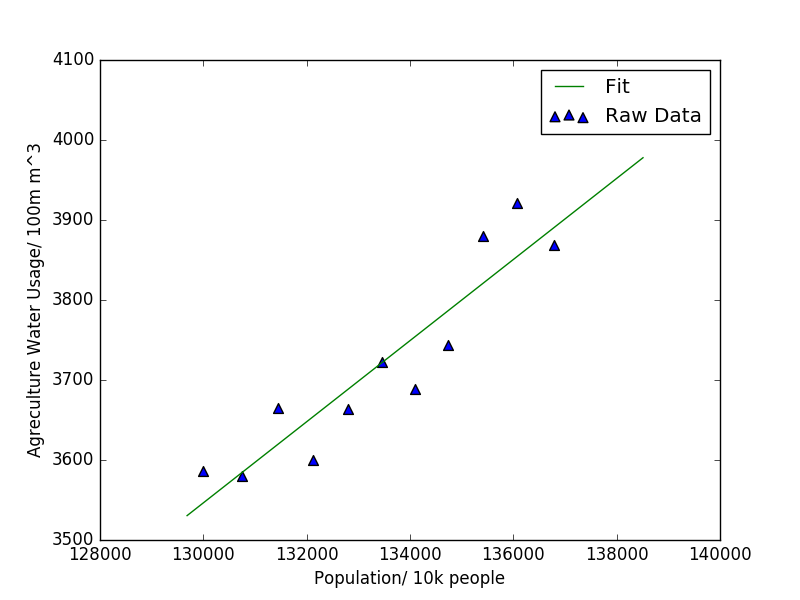
\includegraphics[width = 0.3\textwidth]{picture/Population-Agreculture.png}}
  \subfigure[$\text{PCGDP}$]{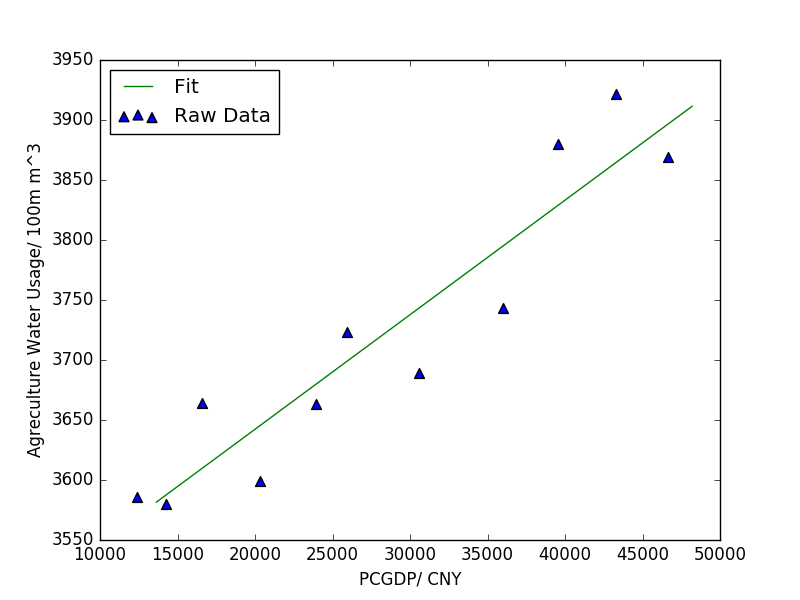
\includegraphics[width = 0.3\textwidth]{picture/PCGDP-Agreculture.png}}
  \subfigure[$\text{IA}$]{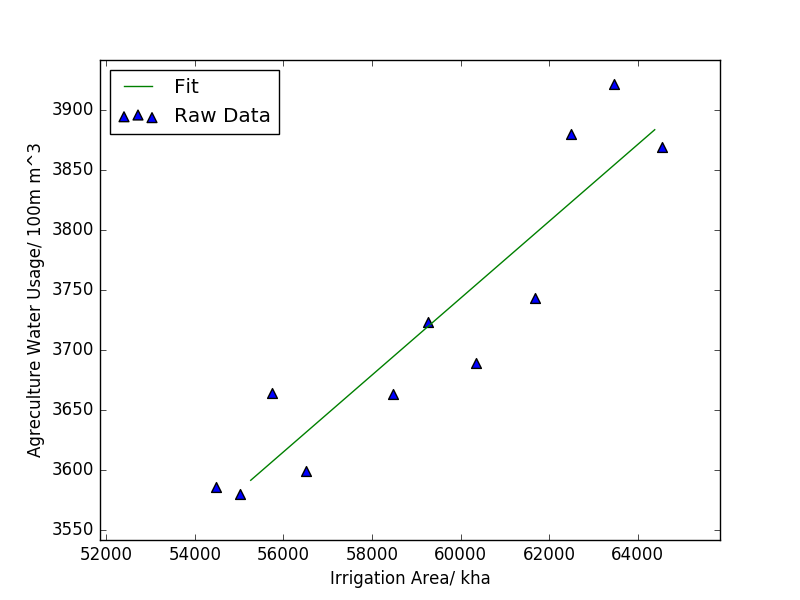
\includegraphics[width = 0.3\textwidth]{picture/IrrigationArea-Agreculture.png}}
  \caption{AWC - parameters}
  \label{fig: AWC para}
  \end{figure}

  \begin{figure}[!h]
  \centering
  \subfigure[$P$]{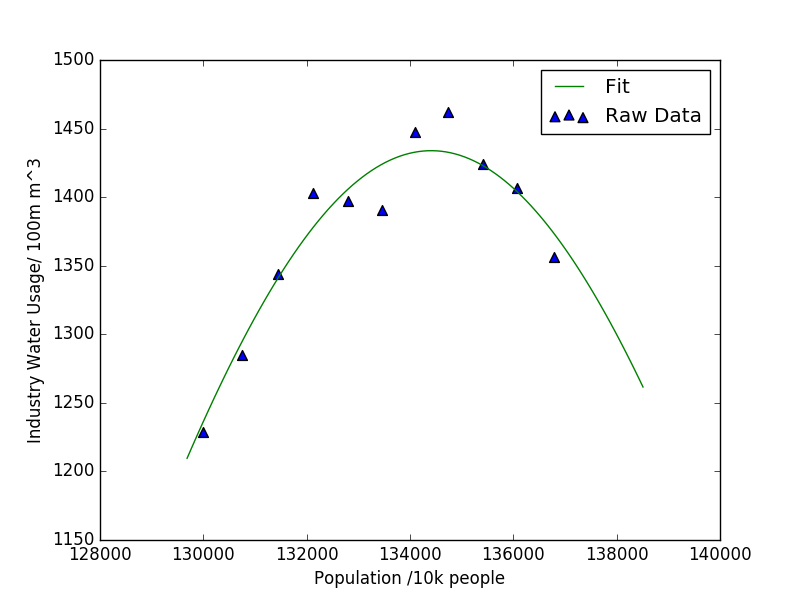
\includegraphics[width = 0.45\textwidth]{picture/Population-Industry.png}}
  \subfigure[$\text{PCGDP}$]{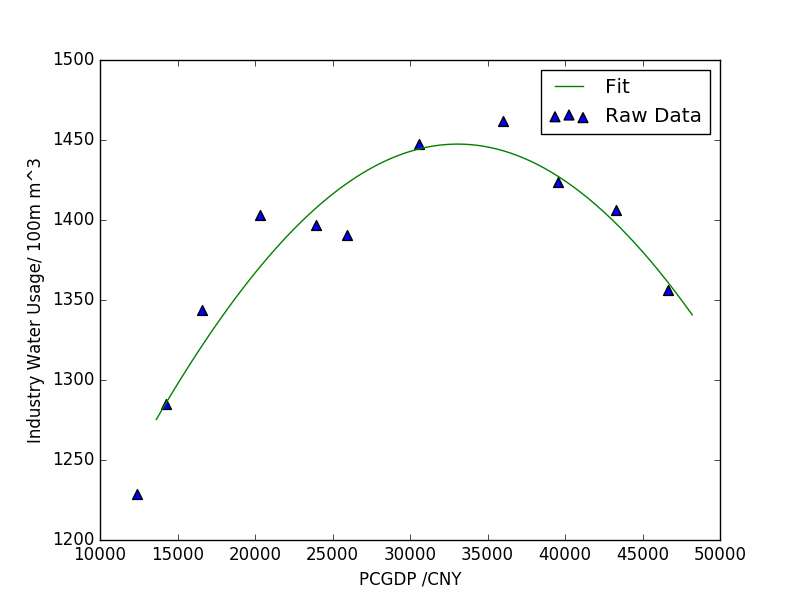
\includegraphics[width = 0.45\textwidth]{picture/PCGDP-Industry.png}}
  \subfigure[$\text{ELP}$]{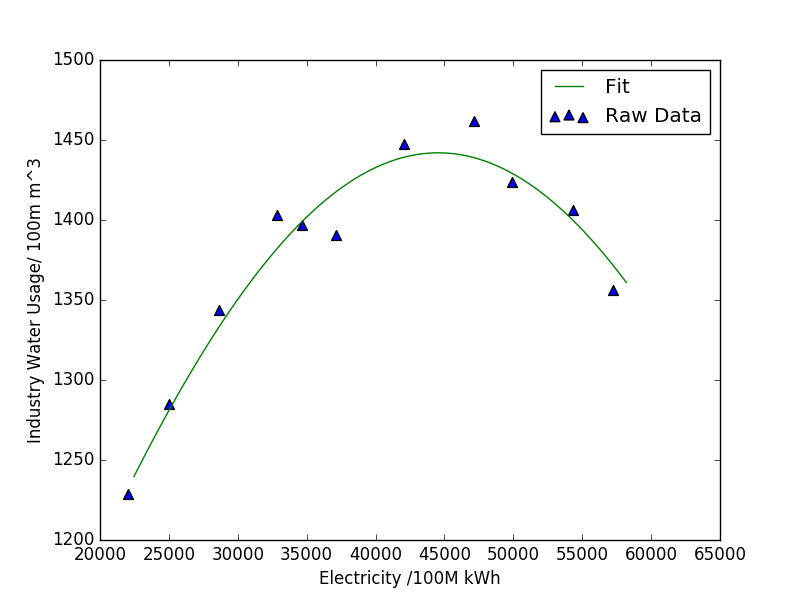
\includegraphics[width = 0.45\textwidth]{picture/Electricity-Industry.png}}
  \subfigure[$\text{ISP}$]{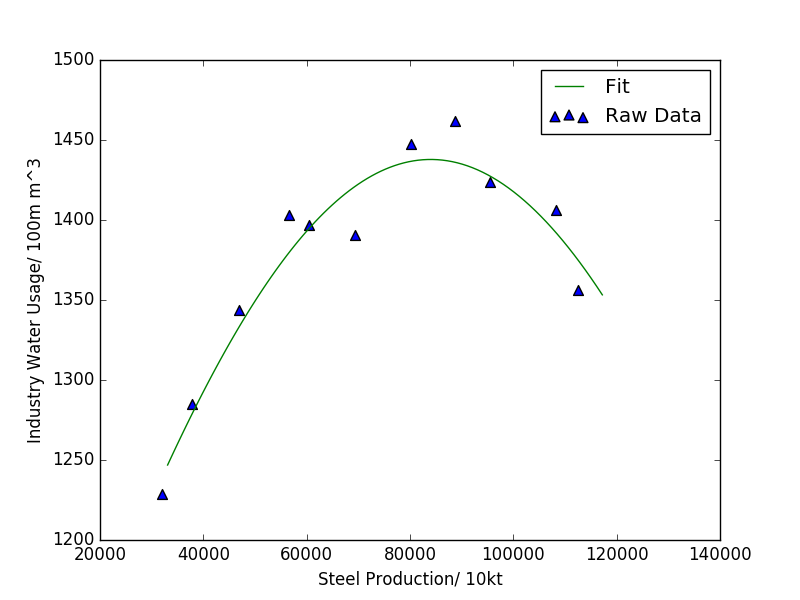
\includegraphics[width = 0.45\textwidth]{picture/SteelProduct-Industry.png}}
  \caption{IWC - parameters}
  \label{fig: IWC para}
  \end{figure}


  \begin{figure}[!h]
  \centering
  \subfigure[$P$]{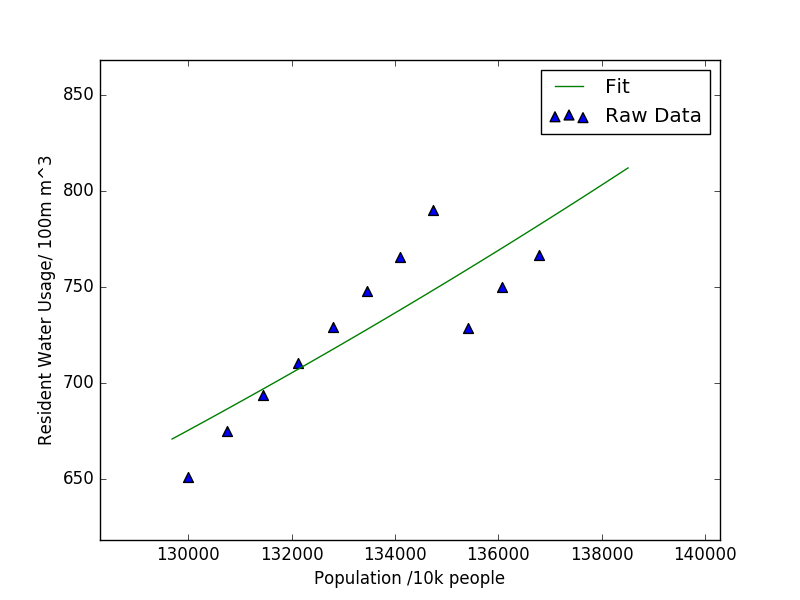
\includegraphics[width = 0.45\textwidth]{picture/Population-Resident.png}}
  \subfigure[$\text{PCGDP}$]{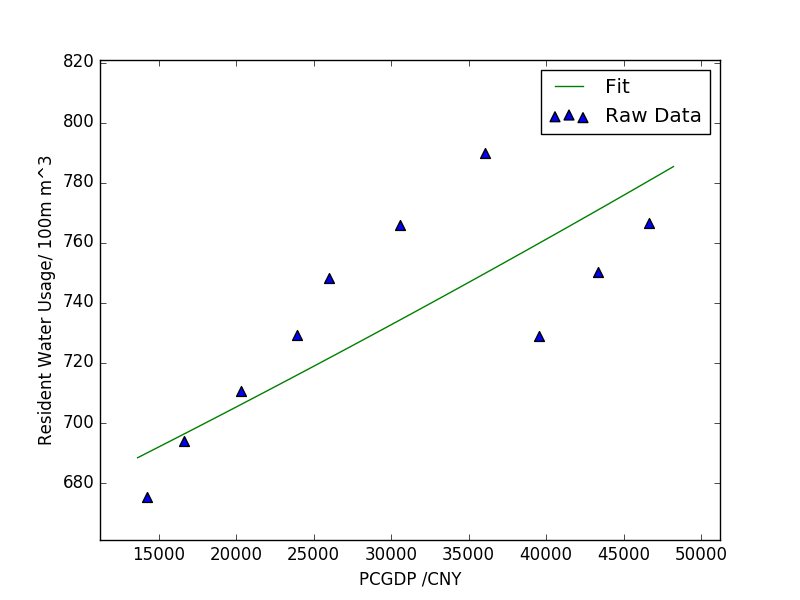
\includegraphics[width = 0.45\textwidth]{picture/PCGDP-Resident.png}}
  \caption{DWC - parameters}
  \label{fig: DWC para}
  \end{figure}


\section{Intervention plan designing}

\section{Prediction with Intervention plan}

\section{Conclusion}


\begin{thebibliography}{99}
  \bibitem{AbilityMeasure} {Falkenmark and Lindh 1976, quoted in UNEP/WMO.Climate Change 2001: Working Group II: Impacts,Adaptation and Vulnerability. UNEP. Retrieved 3 February 2009.}
  \bibitem{WaterCycle} trinityrivertexas.org, Living with the Trinity Lesson Plan 1: The Natural Water Cycle and the Urban Water Cycle
  \bibitem{WaterScarcityMap} http://www.unep.org/dewa/vitalwater
  \bibitem{ChinaDataBase} http://www.stats.gov.cn
  \bibitem{Pearson} https://en.wikipedia.org/wiki/Pearson\_product-moment\_correlation\_coefficient\#Definition
  \bibitem{pearsonr} http://www.statsoft.com/textbook/glosp.html\#Pearson\%20Correlation
  \bibitem{Spearman} https://en.wikipedia.org/wiki/Spearman\%27s\_rank\_correlation\_coefficient
  \bibitem{spearmanr} Zwillinger, D. and Kokoska, S. (2000). CRC Standard Probability and Statistics Tables and Formulae. Chapman \& Hall: New York. 2000. Section 14.7
  \bibitem{ranked variables} Myers, Jerome L.; Well, Arnold D. (2003). Research Design and Statistical Analysis (2nd ed.). Lawrence Erlbaum. p. 508
  \bibitem{Kendall} https://en.wikipedia.org/wiki/Kendall\_rank\_correlation\_coefficient
  \bibitem{kendalltau} W.R. Knight, “A Computer Method for Calculating Kendall’s Tau with Ungrouped Data”, Journal of the American Statistical Association, Vol. 61, No. 314, Part 1, pp. 436-439, 1966

\end{thebibliography}


%==========================================================

\begin{comment}
%===============================appendices===============================
    \begin{appendices}
    %\renewcommand{\thesection}{\Alph{chapter}.}

      \section{First appendix}

    some text...


Here are simulation programmes we used in our model as follow.\\


\textbf{\textcolor[rgb]{0.98,0.00,0.00}{Input matlab source:}}
\lstinputlisting[language=Matlab]{./code/matlab1.m}


      \section{Second appendix}

    some more text\textcolor[rgb]{0.98,0.00,0.00}{\textbf{Input C++ source:}}
\lstinputlisting[language=C++]{./code/sudoku.cpp}

    \end{appendices}

\end{comment}